\section{Begriffe und Elemente}\label{sec:sd-begriffe-und-elemente}

Ein \textbf{Sequenzdiagramm} besteht aus zwei Dimensionen: Die x-Achse beinhaltet die Kommunikationspartner, die y-Achse die \textbf{Lebenslinien} der beteiligten Kommunikationspartner.\\

\noindent
Eine Lebenslinie beginnt mit einem Rechteck, in dem Name und Typ des beteiligten Objektes notiert sind.
An dieser Stelle gilt die in der UML gebräuchliche Notation für Objekte: also \code{[Name]:Typ}, \underline{unterstrichen}.

\subsection{Nachrichten}
Eine \textbf{Nachricht} stellt eine Kommunikation zwischen zwei Objekten dar.\\
Eine Nachricht kann nicht nur für den \textbf{Aufruf} einer Operation auf einem Objekt stehen, sondern auch für eine eingehende \textbf{Antwort}, die von dem Aufrufer erwartet wird.\\
Neben Operationsaufrufen können Nachrichten auch als Signalübermittlung auftreten - diese sind immer \textbf{asynchron}.

\begin{itemize}
    \item \textbf{Synchrone Nachricht}: Eine synchrone Nachricht blockiert den Aufrufer, der bis auf die Antwort des aufgerufenen Objektes warten muss.\\
    Eine synchrone Nachricht wird dargestellt durch eine Linie mit einem geschlossenen Pfeil.
    \item \textbf{asynchrone Nachricht}: Eine asynchrone Nachricht ist eine Nachricht, nach der der Aufrufer nicht blockiert wird, er kann seine Arbeit also fortsetzen.\\
    Asynchrone Nachrichten werden dargestellt durch eine Linie mit einer offenen Pfeilspitze
    \item \textbf{Antworten}: Antwortnachrichten eines Objektes werden durch eine gestrichelte Linie mit offener Pfeilspitze dargestellt. \\
    Die Darstellung von Antwortnachrichten ist optional: Sie sollten nur angegeben werden, wenn ein wichtiger Wert zurückgegeben wird.
\end{itemize}

\noindent
Als Ausgangspunkt einer Nachricht kann eine sog. \textbf{found message} dienen. Eine \textit{found message} ist eine Nachricht, bei der dem Empfänger bekannt ist, die Angabe des Senders aber außerhalb der zu erstellenden Spezifikation liegt.\\
Um einen Endpunkt zu modellieren, kann eine \textbf{lost message} verwendet werden - hierbei liegt der Empfänger außerhelb der Spezifikation  (vgl.~\cite[598]{OMG17}).\\
Die Notation für beide ist in Abbildung~\ref{fig:lost-found-message} dargestellt.

\begin{figure}
    \centering
    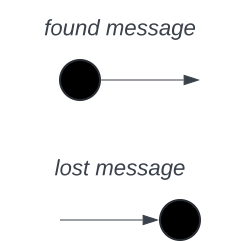
\includegraphics[scale=0.5]{part three/Sequenzdiagramme/img/lost-found-message}
    \caption{Notation einer \textbf{found message} bzw. einer \textbf{found message}. (Quelle: in Anlehnung an \cite[596]{OMG17})}
    \label{fig:lost-found-message}
\end{figure}

\noindent
Nachrichten können \textbf{Argumente} haben, die ggfl. mit den Parametern der angesprochenen Operationen korrespondieren (vgl.~\cite[32]{Buh09}).
Die Syntax lautet wie folgt:

\begin{itemize}
    \item \code{Name[(Argumentliste)]}
    \item \code{*} - falls kein Name definiert werden kann
\end{itemize}

\noindent
Die \code{Argumentliste} ist aufgebaut wie folgt:

\begin{itemize}
    \item \code{([Parametername=]Wert)}
\end{itemize}

\noindent
Als einzelnes Argument kann auch ein Platzhalter in Form eines \textit{Hyphens} (``\code{-}``) angegeben werden: Dies bringt zum Ausdruck, dass kein Wert für einen in der Operation definierten formalen Parameter gefunden werden kann.\\

\noindent
\textbf{Antworten} haben die folgende Syntax:

\medskip
\noindent
\begin{small}
    \textcolor{blue}{[Attributzuweisung]Nachrichtenname[(Argumentliste], [NameRückgabeparameter:Rückgabewert)][:Rückgabewert]}
\end{small}
\noindent

\begin{tcolorbox}[title=Syntax Antworten,colback=red!20]
    Typo bei der Klammerung in ~\cite[32]{Buh09} wie o.a.\\
    Die Korrekte Syntax lautet:

    \begin{small}
        \textcolor{blue}{
            [<assignment-target> ‘=’] <message-name>
            [‘(’ [<output-argument-list>] ‘)’] [‘:’ <value-specification>]
        }
    \end{small}
    Für weitere Informationen s. \cite[577 f.]{OMG17}

\end{tcolorbox}


\subsection*{Aktionssequenzen}
Auf den Lebenslinien der Kommunikationspartner werden \textbf{Aktionssequenzen} dargestellt: Auf der Ebene von Objekten ist eine Aktionssequenz der Ablauf einer Methode, die durch eine Nachricht (Operationsaufruf) gestartet und durch eine Antwort oder ihre Abarbeitung (asynchroner Aufruf) beendet wird.

\subsubsection*{Zustandsbedingung}
\textbf{Zustandsbedingungen} können ebenfalls an den Lebenslinien notiert werden: Diese müssen erfüllt sein, damit ein Teilnehmer Nachrichten empfangen bzw. versenden kann (s. Abbildung~\ref{fig:stateinvariant}).

\begin{figure}
    \centering
    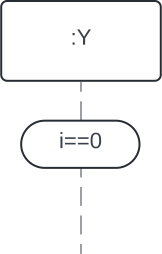
\includegraphics[scale=0.5]{part three/Sequenzdiagramme/img/stateinvariant}
    \caption{Angabe einer Zustandsbedingung unter Verwendung einer \textbf{StateInvariant}-Elements. (Quelle: in Anlehnung an \cite[597]{OMG17})}
    \label{fig:stateinvariant}
\end{figure}

\noindent
Kommunikationspartner können erzeugt (\textbf{creation event}) und zerstört werden (\textbf{destruction event}), wodurch die Erzeugung und das Zerstören bspw. von Objekten im Interaktionsrahmen ausgedrückt wird.
Bei dem Zerstören eines Objektes wird an seine Lebenslinie ein \textbf{DestructionOccurrenceSpecification symbol} notiert, welches die gestalt eines "X" hat (vgl.~\cite[578]{OMG17}).

\begin{tcolorbox}[title=creation event, colback=white]
    Eine Nachricht, die das Erzeugen eines Objektes bewirkt, hat eine gestrichelte Linie und und eine offene Pfeilspitze (vgl~\cite[577]{OMG17})
\end{tcolorbox}

\subsection{Kombinierte Fragmente}
Sequenzdiagramme können Interaktionsrahmen oder auch \textbf{kombinierte Fragmente} darstellen.\\
Interaktionsrahmen bestehen aus einem \textbf{Interaktionsoperator} und einem oder mehreren \textbf{Interaktionsoperanden} (vgl.~\cite[582]{OMG17}).\\
Der Name des Operators wird in der linken oberen Ecke des Interaktionsrahmen angegeben (s. Abbildung ~\ref{fig:interaktionsoperand}).\\
Folgende Bezeichner können für den Operator angegeben werden (vgl.~\cite[583]{OMG17}):

\begin{itemize}
    \item \code{alt} - es können mehrere alternative Abläufe definiert werden
    \item \code{loop} - mehrere Ausführungen, die von einer Bedingung gesteuert werden
    \item \code{opt} - Ausführung, wenn eine geg. Bedingung zutrifft
    \item \code{par} - fragment läuft parallel
\end{itemize}

\begin{figure}
    \centering
    
\includegraphics[scale=0.5]{part three/Sequenzdiagramme/img/interaktionsoperand}
    \caption{Kombiniertes Fragment mit dem Operator \textbf{loop} und dem Operanden $i < 10$. (Quelle: eigene)}
    \label{fig:interaktionsoperand}
\end{figure}

\begin{tcolorbox}[title=Syntax Antworten,colback=red!20]
    Typo bei Operatorenname in ~\cite[34]{Buh09}:
    Statt \textbf{op} muss es \textbf{opt} lauten.
\end{tcolorbox}

\subsection{Interaktionsreferenz}

\textbf{Interaktionsreferenzen} erlauben das Wiederverwenden vollständiger Interaktionsdiagramme.\\
Zur Kennzeichnung einer Interaktionsreferenz wird das Kürzel \code{ref} verwendet.\\
Die Signatur eines Interaktionsrahmens kann dann erweitert werden:\\

\noindent
\code{Name[Parameterliste][:Rückgabetyp]}\\

\blockquote[{\cite[35]{Buh09}}]{
Bei der Verwendung eines Interaktionsrahmens mit definierten Parametern müssen dann die notwendigen Argumente Übergeben werden.
}

Für ein Beispiel s. Abbildung~\ref{fig:interaktionsreferenz}.

\begin{figure}
    \centering
    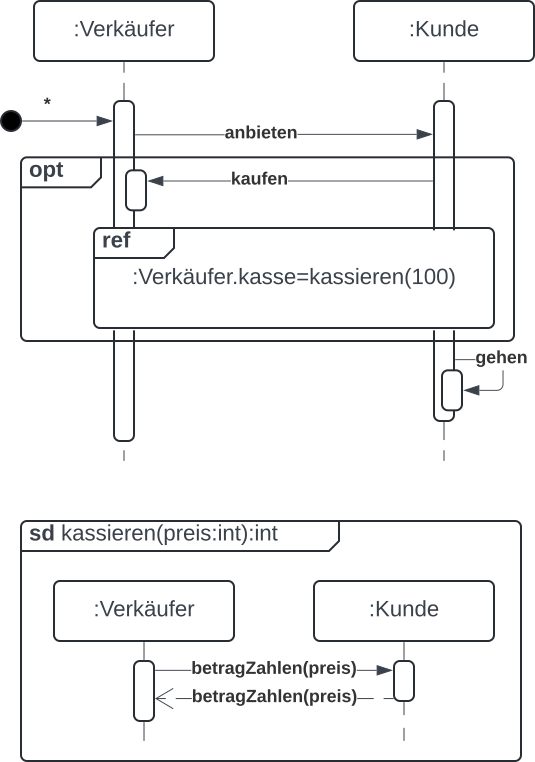
\includegraphics[scale=0.5]{part three/Sequenzdiagramme/img/interaktionsreferenz}
    \caption{Sequenzdiagramm mit einem referenzierten Interaktionsrahmen. (Quelle: in Anlehnung an \cite[35]{Buh09})}
    \label{fig:interaktionsreferenz}
\end{figure}